\section{Hardware Components and Construction}

\subsection{Cooling and air purging system}

The SVT regions are cantilevered off a chilled cold plate that is designed to remove the heat generated by the electronics and provide operational  conditions for the sensors. External cooling has been chosen over internal cooling (tubes in the modules) to keep the amount of material in the active area as low as possible. Front-end electronics is producing 5 watts per module ? 42 total modules producing 210 watts. The HFCBs are routed through a 10 mm slots in the cold plate. The cold plate, (see Fig.~\ref{fig:coldplate}), includes a copper plate with brazed quarter inch copper tubes and PEEK plate on the upstream side. 

\begin{figure}[hbt] 
\centering 
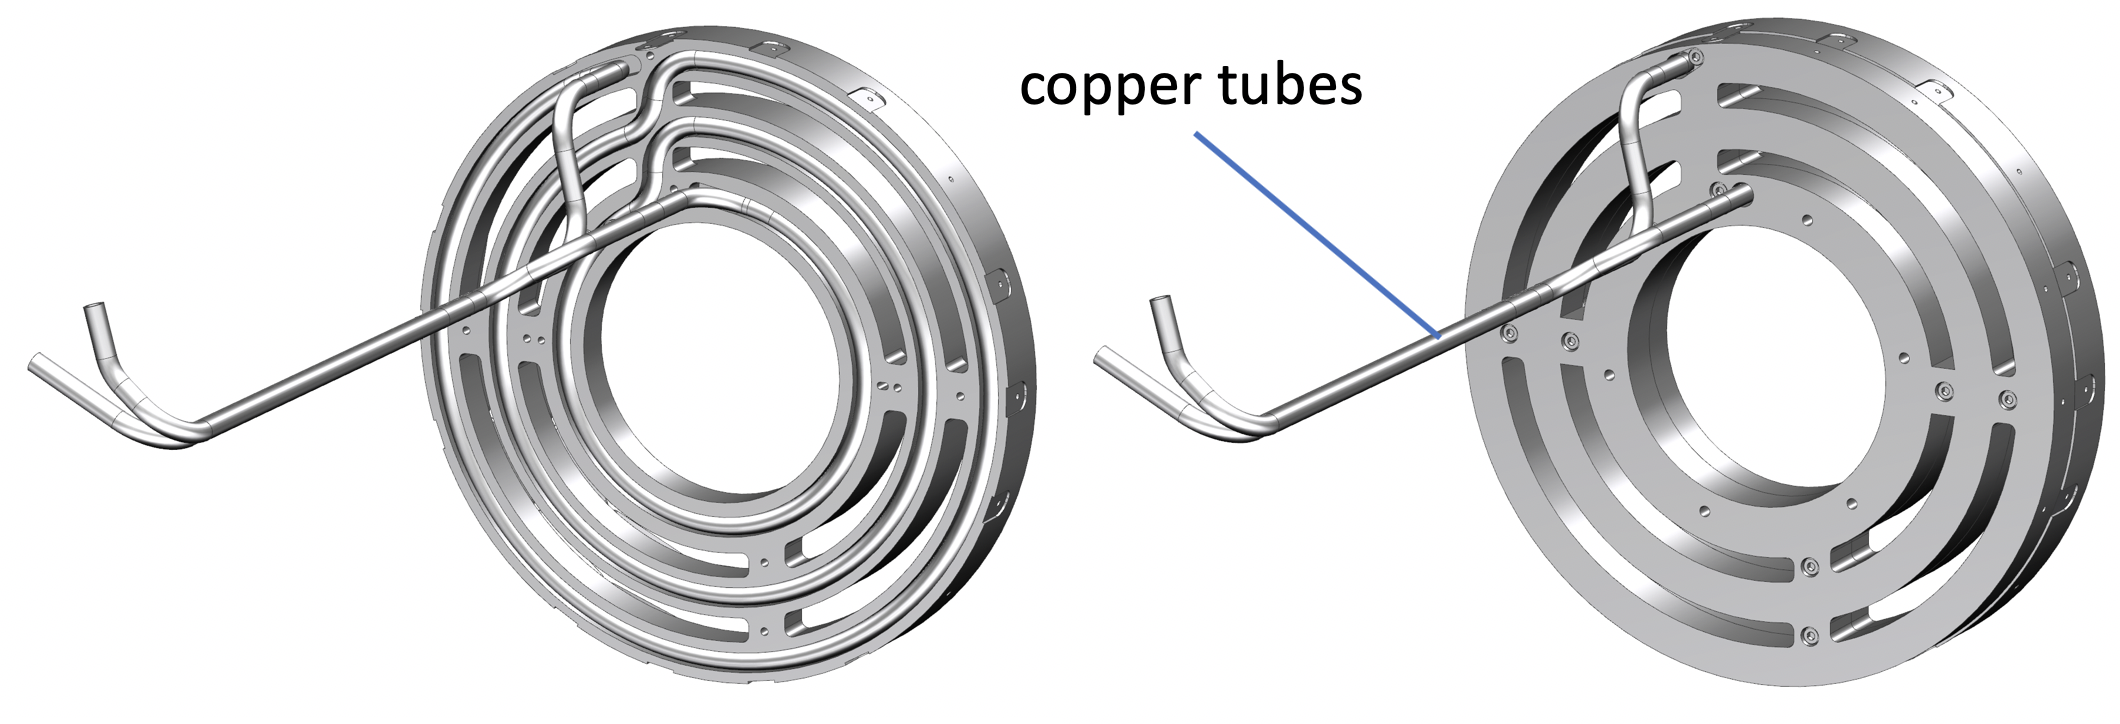
\includegraphics[width=1.0\columnwidth,keepaspectratio]{coldplate.png}
\caption{Copper tubing furnace brazed to copper cold plate (left), assembled cold plate (right).}
\label{fig:coldplate}
\end{figure}

%\begin{wrapfigure}{l}{0.5\columnwidth}
%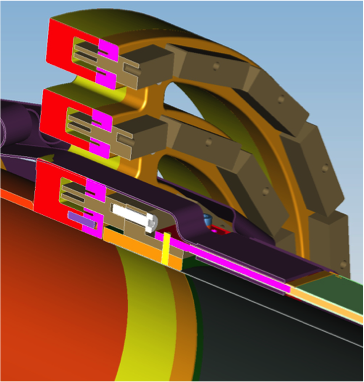
\includegraphics[width=0.5\columnwidth]{cold_plate.png}
%\caption{Routing flex cable through the cold plate.}
%\label{fig:cold-plate}
%\end{wrapfigure}

Coolant is 50/50 ethylene glycol and water is flowing at 2 liters per minute at a temperature of -20$\degree$C.
Coldplate including plastic upstream cover made from PEEK plastic. HFCB ribbon cables also go through the slots.
Dry air flowing through the slots in the cold plate is cooled by the liquid coolant circulating in the tube inside the air purging line (see Fig.~\ref{fig:purging1}). 

\begin{figure}[hbt] 
\centering 
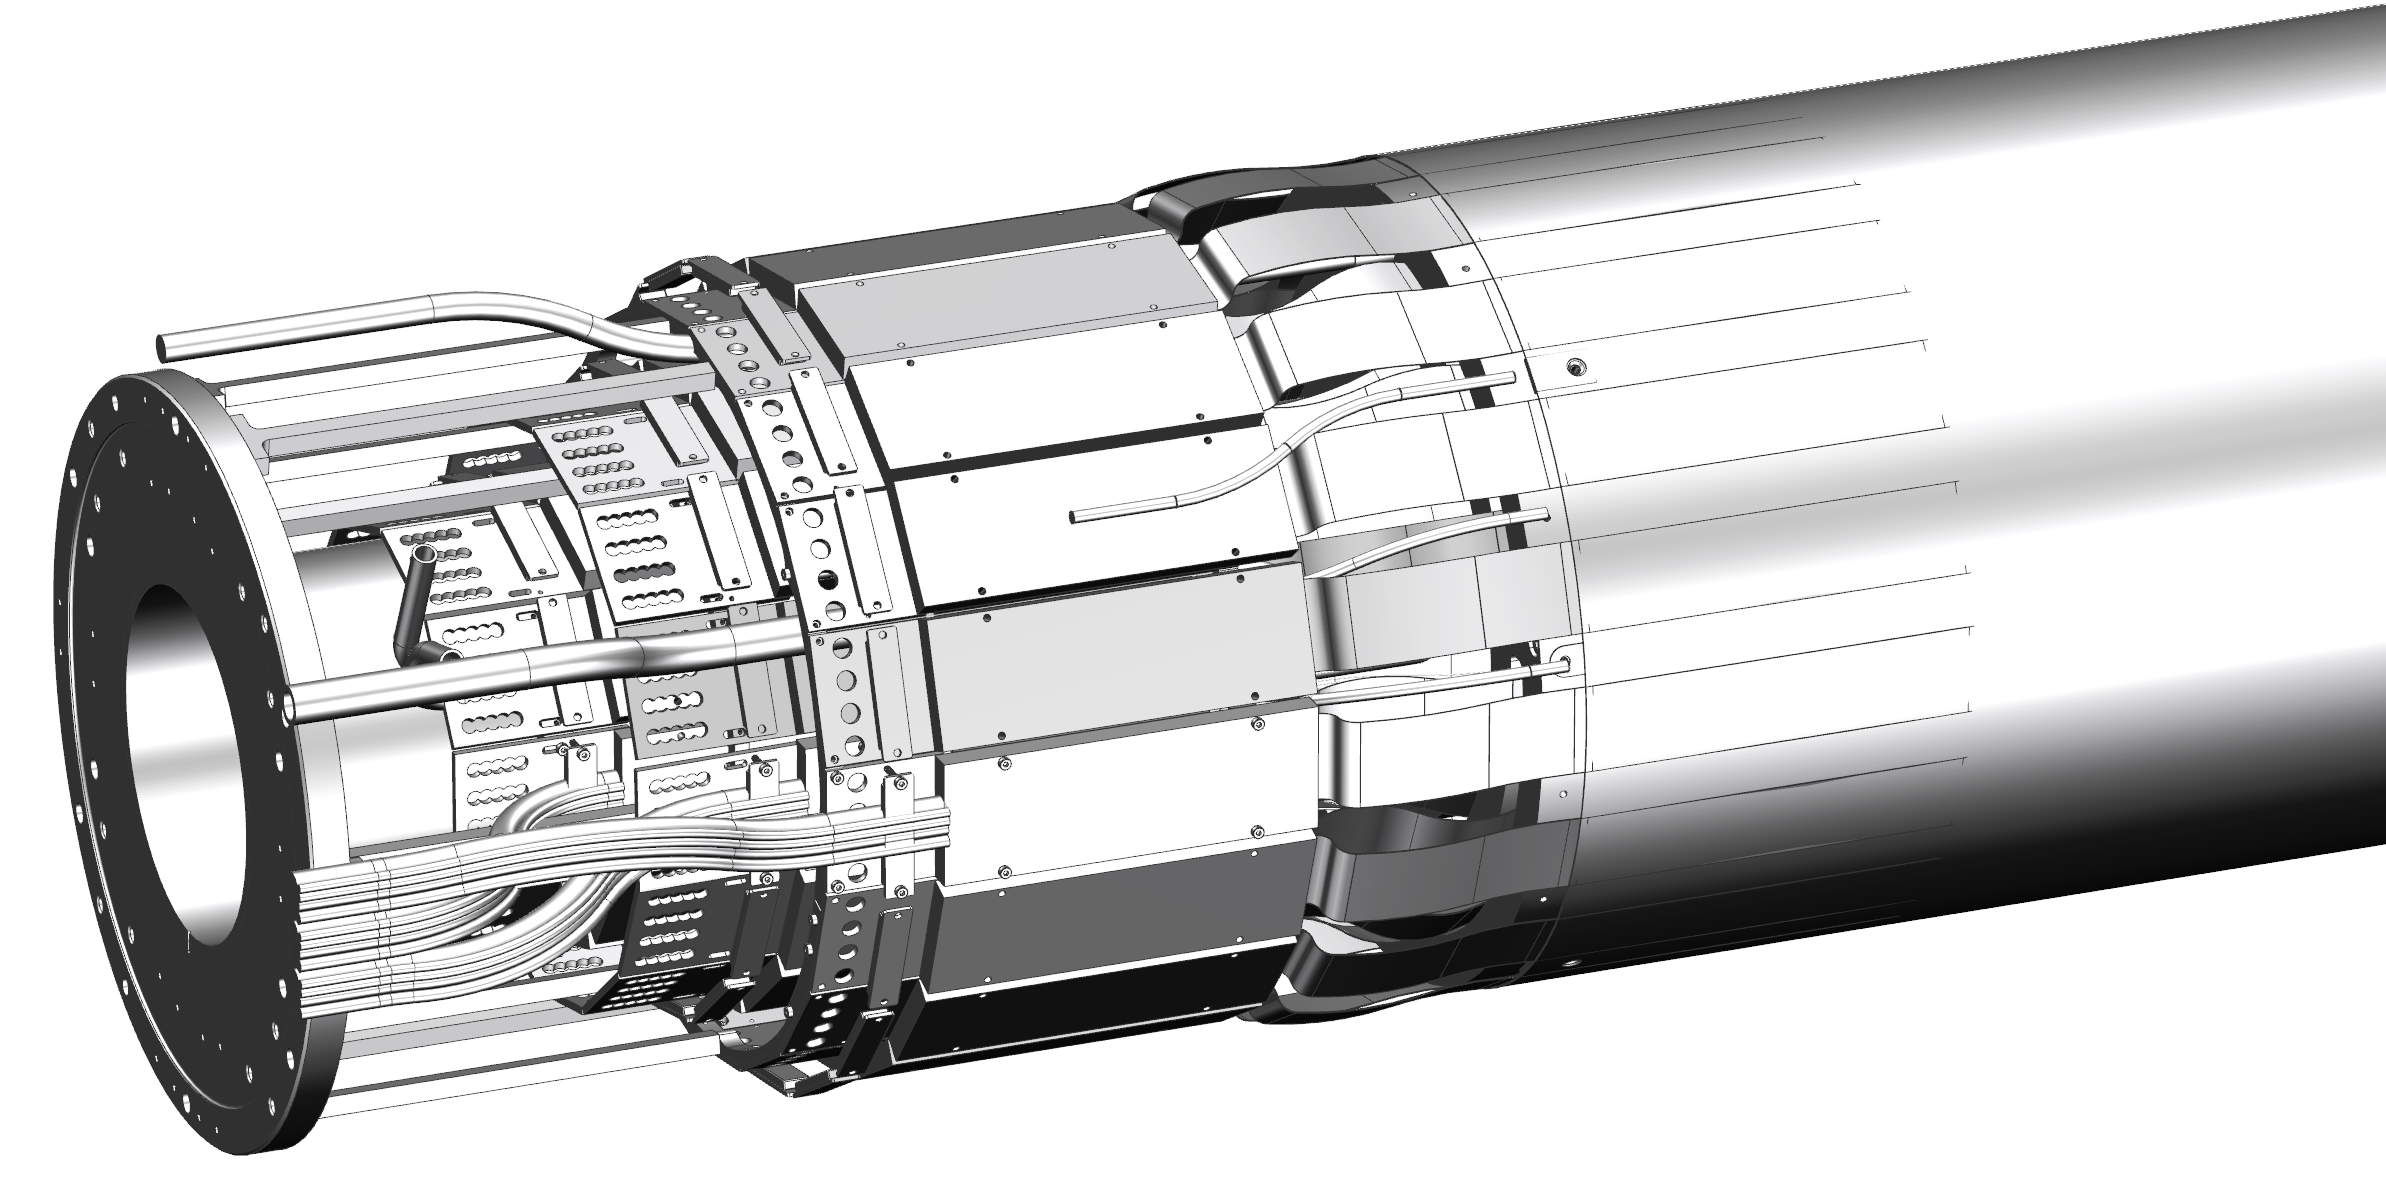
\includegraphics[width=1.0\columnwidth,keepaspectratio]{purging1.png}
\caption{Dry air flows past connectors, through slots in cold plate, into Faraday cage, past sensors, and out cover holes.}
\label{fig:purging1}
\end{figure}

With 100 liters per minute of chilled air flow across the cold plate, the sensors are cooled to the operational temperature of -10$\degree$C. The Faraday cage cap on the downstream end has 4 holes to ensure the flow of cold air along the barrel. 

\begin{figure}[hbt] 
\centering 
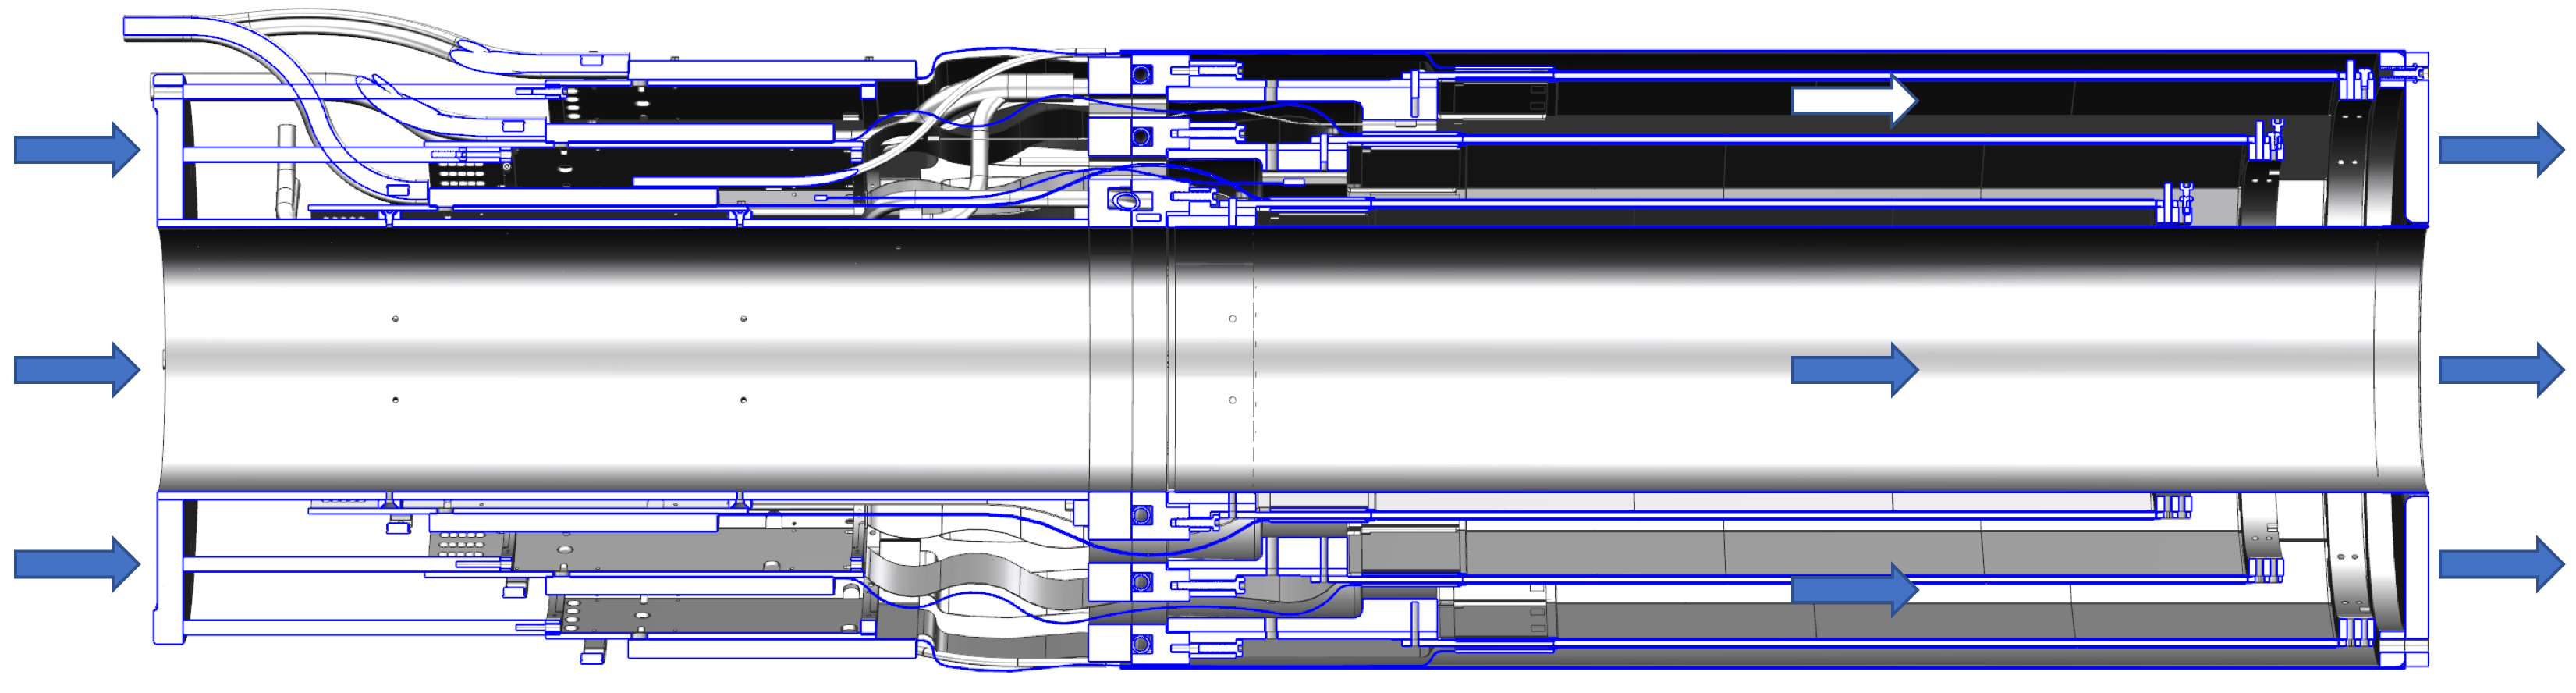
\includegraphics[width=1.0\columnwidth,keepaspectratio]{purging2.png}
\caption{Cross Section of SVT Detector.  Dry air flow in yellow.}
\label{fig:purging2}
\end{figure}

Outside of Faraday Cage is insulated with 3 mm thick neoprene sheet. Barrel is protected from environment humidity by purging dry air between the scattering chamber and the inner shell of the Faraday cage and between the outer shell of the Faraday cage and the protective plastic cover (see Fig.~\ref{fig:purging2}). 

\subsection{Slow controls, interlocks, and monitoring, detector safety}

Ambient conditions inside the detector are monitored by temperature and humidity sensors installed inside the downstream rings. 
Safe operation of the tracker is ensured by the dedicated monitoring of all important operation parameters including monitoring of low and high voltages and currents, temperatures and dew points. To avoid condensation the detector volume is purged with nitrogen. EPICS based slow control and monitoring system has been developed. Software and hardware interlocks continuously monitor critical system parameters. The performance and stability of the system is tested at various operation temperatures. Sensor leakage currents are below 400 nA with coolant at -20$\degree$C. Humidity inside the barrel is about 2~$\%$.

%\begin{figure}[hbt] 
%\centering 
%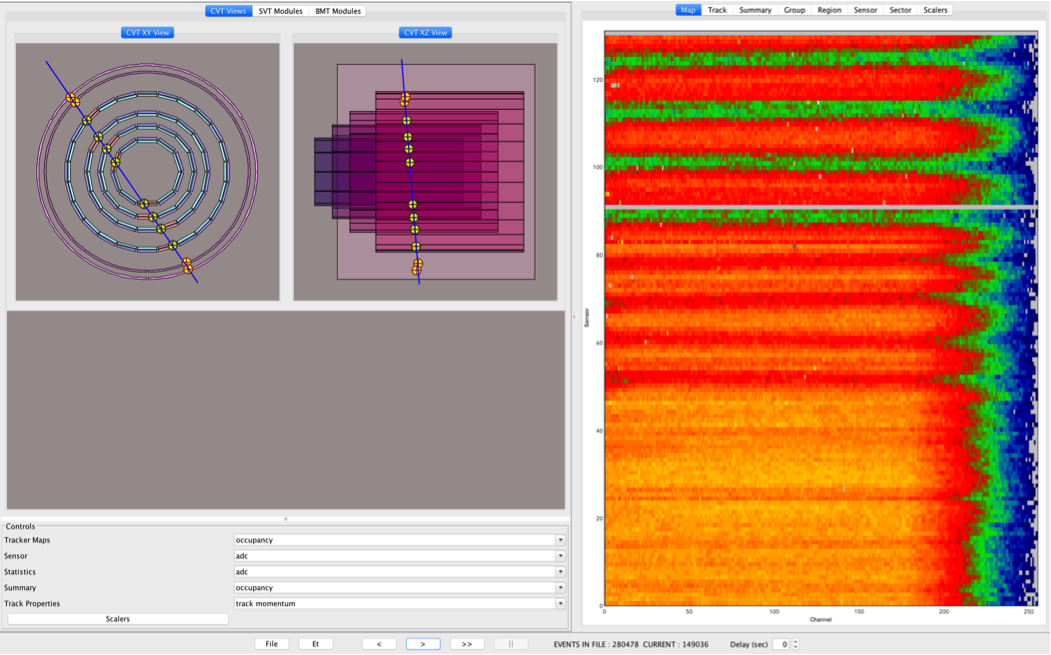
\includegraphics[width=0.9\columnwidth,keepaspectratio]{occupancy-map.png}
%\caption{Online monitoring of the SVT}
%\label{fig:monitoring}
%\end{figure}

Java based data quality monitoring tools were developed to check the quality of the data both online and offline. 
%Online SVT monitoring interface is shown in Fig.~\ref{fig:monitoring}. The tools allow the shifter to check the status of the track reconstruction and performance of the individual modules. On the left side of the interface are shown the event display and the histogram selection menus. On the right side there are canvases for the selected groups of histograms. The hit occupancy canvas is selected.

